\documentclass[tikz,border=3pt]{standalone}
\usepackage{pgfplots}
\pgfplotsset{compat=1.18}
\begin{document}
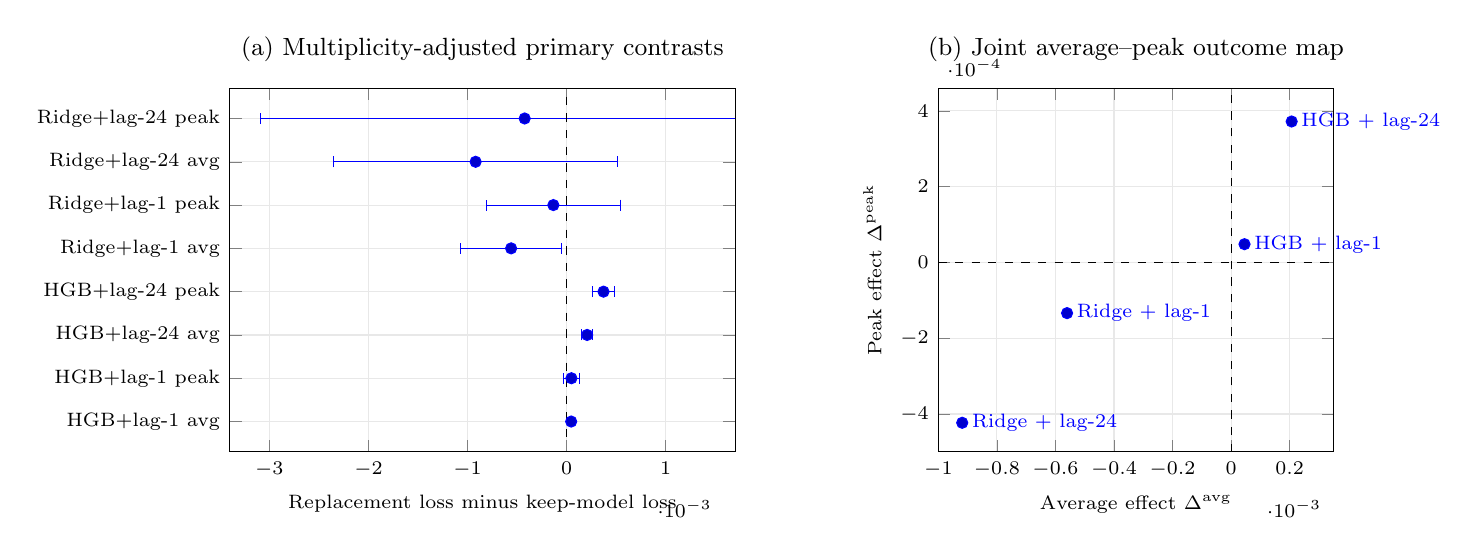
\begin{tikzpicture}[font=\sffamily\small]
\begin{axis}[
  width=8.0cm,height=6.2cm,
  xmin=-0.0034,xmax=0.0017,
  xlabel={Replacement loss minus keep-model loss},
  ytick={1,2,3,4,5,6,7,8},
  yticklabels={Ridge+lag-24 peak,Ridge+lag-24 avg,Ridge+lag-1 peak,Ridge+lag-1 avg,HGB+lag-24 peak,HGB+lag-24 avg,HGB+lag-1 peak,HGB+lag-1 avg},
  y dir=reverse,
  title={(a) Multiplicity-adjusted primary contrasts},
  grid=major,grid style={gray!18},
  tick label style={font=\scriptsize},label style={font=\scriptsize},title style={font=\small}
]
\addplot+[only marks,mark=*,error bars/.cd,x dir=both,x explicit] coordinates {
 (-0.0004233,1) +- (0.0026682,0.0018311)
 (-0.0009185,2) +- (0.0014331,0.0015105)
 (-0.0001338,3) +- (0.0006771,0.0005382)
 (-0.0005603,4) +- (0.0005071,0.0004202)
 (0.0003721,5) +- (0.0001138,0.0001831)
 (0.0002070,6) +- (0.0000547,0.0000696)
 (0.0000482,7) +- (0.0000831,0.0001388)
 (0.0000459,8) +- (0.0000156,0.0000143)
};
\draw[dashed] (axis cs:0,0.5) -- (axis cs:0,8.5);
\end{axis}

\begin{axis}[
  xshift=9.0cm,
  width=6.6cm,height=6.2cm,
  xmin=-0.0010,xmax=0.00035,
  ymin=-0.0005,ymax=0.00046,
  xlabel={Average effect $\Delta^{\mathrm{avg}}$},
  ylabel={Peak effect $\Delta^{\mathrm{peak}}$},
  title={(b) Joint average--peak outcome map},
  grid=major,grid style={gray!18},
  tick label style={font=\scriptsize},label style={font=\scriptsize},title style={font=\small}
]
\draw[dashed] (axis cs:0,-0.0005) -- (axis cs:0,0.00046);
\draw[dashed] (axis cs:-0.0010,0) -- (axis cs:0.00035,0);
\addplot+[only marks,mark=*,nodes near coords,point meta=explicit symbolic,every node near coord/.append style={font=\scriptsize,anchor=west}] coordinates {
 (0.0000459,0.0000482) [HGB + lag-1]
 (0.0002070,0.0003721) [HGB + lag-24]
 (-0.0005603,-0.0001338) [Ridge + lag-1]
 (-0.0009185,-0.0004233) [Ridge + lag-24]
};
\end{axis}
\end{tikzpicture}
\end{document}
